% Created 2019-09-22 Sun 19:43
% Intended LaTeX compiler: pdflatex
\documentclass[nobib]{tufte-handout}


\usepackage{minted}
\usepackage{ifluatex, ifxetex}
%Next block avoids bug, from http://tex.stackexchange.com/a/200725/1913
\ifx\ifxetex\ifluatex\else
\newcommand{\textls}[2][5]{%
\begingroup\addfontfeatures{LetterSpace=#1}#2\endgroup
}
\renewcommand{\allcapsspacing}[1]{\textls[15]{#1}}
\renewcommand{\smallcapsspacing}[1]{\textls[10]{#1}}
\renewcommand{\allcaps}[1]{\textls[15]{\MakeTextUppercase{#1}}}
\renewcommand{\smallcaps}[1]{\smallcapsspacing{\scshape\MakeTextLowercase{#1}}}
\renewcommand{\textsc}[1]{\smallcapsspacing{\textsmallcaps{#1}}}
\fi
\usepackage{fontspec}
\setmainfont{ETBookOT}
\setmonofont[Scale=0.8]{Fantasque Sans Mono}
\renewcommand{\contentsname}{contents}
\titleformat{\chapter}%
[display]% shape
{\relax\ifthenelse{\NOT\boolean{@tufte@symmetric}}{\begin{fullwidth}}{}}% format applied to label+text
{\huge\thechapter}% label
{0pt}% horizontal separation between label and title body
{\huge\rmfamily}% before the title body
[\ifthenelse{\NOT\boolean{@tufte@symmetric}}{\end{fullwidth}}{}]% after the title body
\titleformat{\section}%
[hang]% shape
{\normalfont\Large}% format applied to label+text
{\thesection}% label
{1em}% horizontal separation between label and title body
{}% before the title body
[]% after the title body
\titleformat{\subsection}%
[hang]% shape
{\normalfont\large\itshape}% format applied to label+text
{\thesubsection}% label
{1em}% horizontal separation between label and title body
{}% before the title body
[]% after the title body
\renewcommand{\maketitle}{%
\begingroup
\setlength{\parindent}{0pt}%
\setlength{\parskip}{4pt}%
\LARGE\scshape\plaintitle\par
\Large\itshape\plainauthor\par
\Large\itshape\thedate\par
\endgroup
%\thispagestyle{plain}% suppress the running head
%\tuftebreak
%\@afterindentfalse\@afterheading% suppress indentation of the next paragraph
}
\usepackage{graphicx}
\author{james gilles}
\date{september 22 2019}
\title{18.337 homework 0}
\hypersetup{
 pdfauthor={james gilles},
 pdftitle={18.337 homework 0},
 pdfkeywords={},
 pdfsubject={},
 pdfcreator={Emacs 26.3 (Org mode 9.2.6)}, 
 pdflang={English}}
\begin{document}

\maketitle
\tableofcontents


\section{problem 1}
\label{sec:org6b6b449}

This was fairly straightforward; I just followed the instructions in the README. I chose to use SLURM to run my code because I'm more familiar with it.

\begin{minted}[frame=lines,linenos=true,mathescape,breaklines=true]{julia}
$ sbatch submit_forkjoin.sh
$ cat top5norm_forkjoin.log-442748
connecting to worker 1 out of 13
connecting to worker 2 out of 13
connecting to worker 3 out of 13
connecting to worker 4 out of 13
connecting to worker 5 out of 13
connecting to worker 6 out of 13
connecting to worker 7 out of 13
connecting to worker 8 out of 13
connecting to worker 9 out of 13
connecting to worker 10 out of 13
connecting to worker 11 out of 13
connecting to worker 12 out of 13
connecting to worker 13 out of 13
Added workers: 13
Pair{String,Float64}["cavorite"=>1.0; "mooncalf"=>1.0; "lunar"=>1.0; "cavor"=>1.0; "selenites"=>1.0]
Pair{String,Float64}["leblanc"=>1.0; "holsten"=>1.0; "fowler"=>1.0; "brissago"=>1.0; "karenin"=>1.0]
Pair{String,Float64}["montgomery"=>1.0; "puma"=>1.0; "moreau"=>1.0; "prendick"=>1.0; "swine"=>0.964286]
Pair{String,Float64}["withered"=>0.692308; "candles"=>0.619048; "candle"=>0.567568; "shade"=>0.296296; "room"=>0.0686275]
Pair{String,Float64}["psychologist"=>1.0; "morlocks"=>1.0; "weena"=>1.0; "filby"=>1.0; "sphinx"=>1.0]
Pair{String,Float64}["artilleryman"=>1.0; "ulla"=>1.0; "martian"=>1.0; "woking"=>1.0; "martians"=>0.993939]
Pair{String,Float64}["henfrey"=>1.0; "adye"=>1.0; "mariner"=>1.0; "griffin"=>1.0; "jaffers"=>1.0]
Pair{String,Float64}["vee"=>1.0; "ann"=>1.0; "alice"=>1.0; "miniver"=>1.0; "veronica"=>1.0]
Pair{String,Float64}["graham"=>1.0; "aeropile"=>1.0; "howard"=>1.0; "asano"=>1.0; "isbister"=>1.0]
Pair{String,Float64}["smallways"=>1.0; "edna"=>1.0; "germans"=>1.0; "bert"=>1.0; "butteridge"=>1.0]
Pair{String,Float64}["boomfood"=>1.0; "cossar"=>1.0; "hickleybrow"=>1.0; "wondershoot"=>1.0; "herakleophorbia"=>1.0]
Pair{String,Float64}["dad"=>1.0; "slim"=>1.0; "industrialist"=>1.0; "explorer"=>0.956522; "astronomer"=>0.953488]
Pair{String,Float64}["polly"=>1.0; "johnson"=>1.0; "rumbold"=>1.0; "fishbourne"=>1.0; "parsons"=>1.0]
\end{minted}


\section{problem 2}
\label{sec:orgba0ba97}

I decided I wanted to plot the output, colorizing each random walk by hostname. So I brought in DataFrames, to feed to Gadfly after the run was complete.

\marginnote[4in]{I originally tried to use the \texttt{gethostname()} Julia function, but it always returned the same answer from all nodes, possibly because of SLURM messing with environment variables. Using the actual \texttt{`hostname`} command worked, though.}

\begin{minted}[frame=lines,linenos=true,mathescape,breaklines=true]{julia}
println("booting julia...")
using ClusterManagers, Distributed
using DataFrames, CSV
println("done.")

println("demanding workers from slurm...")
addprocs(SlurmManager(parse(Int,ENV["SLURM_NTASKS"])-1))
println("done. added workers: ", nworkers())

println("prepping computation...")
@everywhere begin
    using Random

    # brownian motion
    make_brownian(dt,n) = cumsum([0;sqrt(dt).*randn(n+1)])

    # get the walk for some seed, and grab the hostname as well
    get_results(seed) = begin
        Random.seed!(seed)
        brownian = make_brownian(1, 100)
        hostname = chomp(read(`hostname`, String))
        (brownian, hostname)
    end
end
println("computation prepared.")

println("running...")
seeds = 1:50
results = pmap(get_results, seeds)
println("done.")

println("writing output...")
function format_results(results :: Array{Tuple{Array{Float64, 1}, String}, 1})
    # bundle all outputs into a single dataframe
    all = DataFrame(time = [], y = [], hostname = [])
    for (walk, hostname) in results
        current = DataFrame(time = 1:length(walk), y = walk, hostname = [hostname for i in 1:length(walk)])
        append!(all, current)
    end
    all
end

CSV.write("results.csv", format_results(results))
println("done.")

\end{minted}

The batch script was also very simple.

\marginnote[1in]{I added an \texttt{`-N`} flag to force slurm to actually give me multiple nodes. Otherwise it would schedule most processes onto a single node.}

\begin{minted}[frame=lines,linenos=true,mathescape,breaklines=true]{bash}
#!/bin/sh

#SBATCH -o p2.log-%j
#SBATCH -n 10
#SBATCH -N 10

source /etc/profile
module load julia-1.0
julia p2.jl

\end{minted}

After running that, I copied \texttt{results.csv} over to my machine, and used Gadfly to visualize it:

\begin{minted}[frame=lines,linenos=true,mathescape,breaklines=true]{julia}
import Cairo
using Gadfly, DataFrames, CSV

results = CSV.read("results.csv")

# add groupings to un-confuse lines: 50 runs, 102 steps per run
runs = 50
results[:run] = repeat(1:50, inner=[102])

result = plot(results, x=:time, y=:y, color=:hostname, group=:run, Geom.line)
result |> PNG("results.png", 6.75inch, 4inch, dpi=300)
\end{minted}

\begin{figure*}
\centering
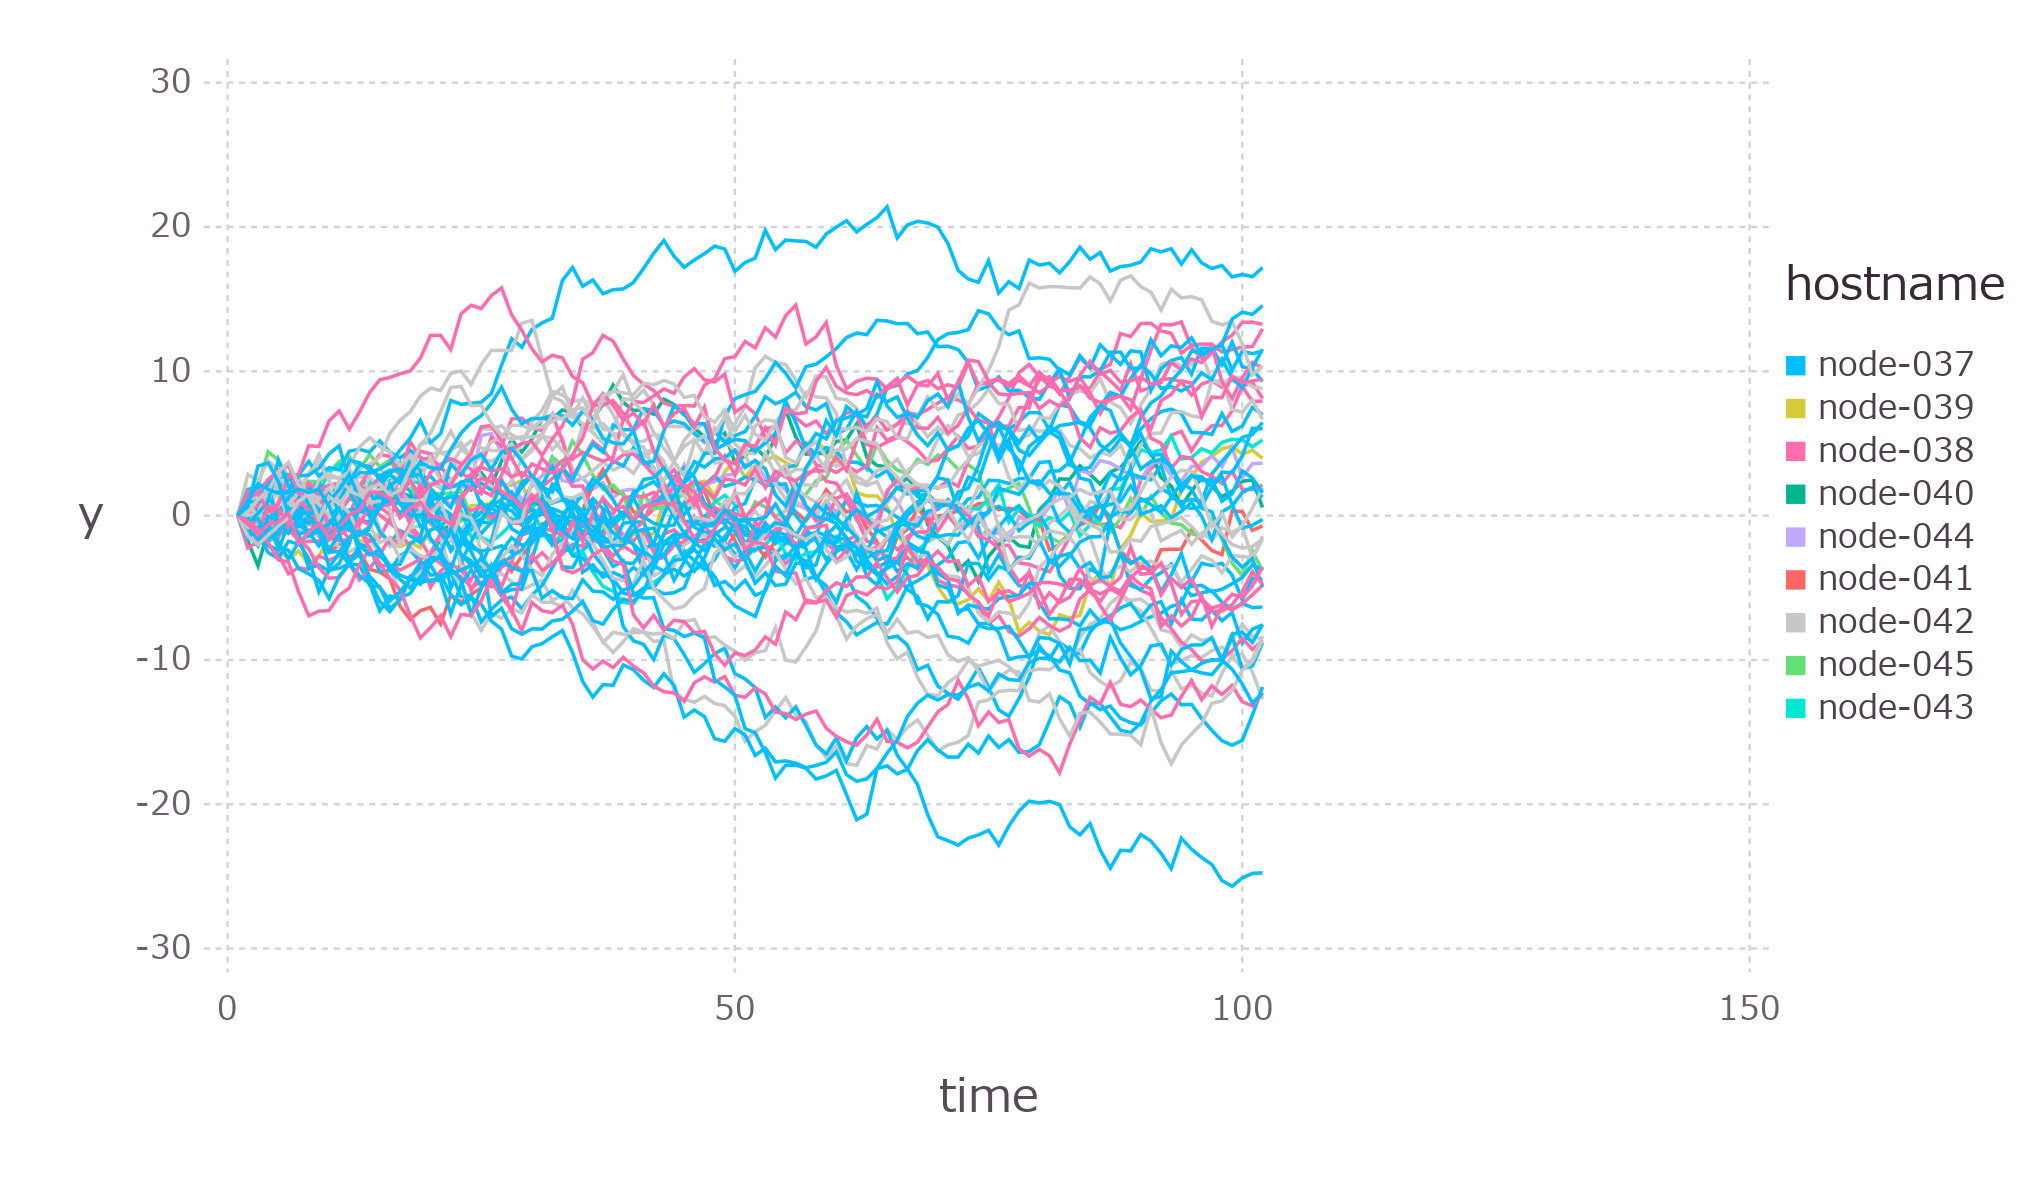
\includegraphics[width=.9\linewidth]{./results.png}
\caption[results]{\label{fig:full-width}
Random walks, colored by hostname.}
\end{figure*}
\end{document}
